\documentclass[12pt,compress,handout]{beamer}  %For printable version
%\documentclass[12pt,compress]{beamer}         %For presentation version

\usepackage{amssymb}
\usepackage{amsmath}
\usepackage{multimedia}
\usepackage{graphicx}
\usepackage{hyperref}
\usepackage{graphicx}


\usetheme{Darmstadt}
\usecolortheme{seahorse} % These 2 lines create a
\usecolortheme{rose}     % toner-friendly handout.

\setbeamertemplate{mini frames}[default]
\setbeamertemplate{sections/subsections in toc}[ball]
\setbeamertemplate{mini frame in other subsection}[default][0]
\setbeamertemplate{frametitle continuation}[from second]

\setbeamersize{<text margin left=0.1 in>, <text margin right=.1 in>,
<sidebar width left=0 in>, <sidebar width right=0 in>}

\setbeamerfont{frametitle}{size=\small}
\setbeamerfont{infolines}{size=\footnotesize}
\setbeamertemplate{footline}[frame number]

\newcounter{thmcnt}
\newtheorem{thm}{Theorem \arabic{thmcnt}}


%%%%%%%%%%%%%%%%%%%%%%%%%%%%%%%%%%%%%%%%%%%%%%%%%%%%%%%%%%%%%%%%%%%%%%%%%%%%%%
% User-defined LaTeX commands
\DeclareMathOperator*{\Cov}{Cov} \DeclareMathOperator*{\Var}{Var}
\DeclareMathOperator*{\argmax}{argmax}
\newcommand{\notorth}{\ensuremath{\perp\!\!\!\!\!\!\diagup\!\!\!\!\!\!\perp}}
\newcommand{\orthog}{\ensuremath{\perp\!\!\!\perp}}
\newcommand{\orth}{\ensuremath{\perp\!\!\!\perp}}


%%%%%%%%%%%%%%%%%%%%%%%%%%%%%%%%%%%%%%%%%%%%%%%%%%%%%%%%%%%%%%%%%%%%%%%%%%%%%%
\begin{document}


%%%%%%%%%%%%%%%%%%%%%%%%%%%%%%%%%%%%%%%%%%%%%%%%%%%%%%%%%%%%%%%%%%%%%%%%%%%%%%%
\title{Sheshinski Specification}

\author{James Heckman\\University of Chicago}

\date{Econ 350\\
This draft, \today}


%%%%%%%%%%%%%%%%%%%%%%%%%%%%%%%%%%%%%%%%%%%%%%%%%%%%%%%%%%%%%%%%%%%%%%%%%%%%%%%
\frame{\titlepage}


%%%%%%%%%%%%%%%%%%%%%%%%%%%%%%%%%%%%%%%%%%%%%%%%%%%%%%%%%%%%%%%%%%%%%%%%%%%%%%%
\section{Basic Sheshinski Specification}
%%%%%%%%%%%%%%%%%%%%%%%%%%%%%%%%%%%%%%%%%%%%%%%%%%%%%%%%%%%%%%%%%%%%%%%%%%%%%%%
\begin{frame}
\begin{center}
\textbf{\insertsection}
\end{center}
\begin{itemize}[<+->]
\item $\beta =1$, $\alpha =1$ in $\dot{H}=AH^{\beta}I^{\alpha}-\sigma H$
\begin{gather*}
\dot{H}=AIH-\sigma H\\
\\
\mathcal{H}: \quad e^{-rt}R(1-I)H+\mu (AIH-\sigma H)
\end{gather*}
\\[2mm]

\item Bang-Bang: $I = 1$ if
\begin{gather*}
\mu(t) AH\geq e^{-rt}RH \\
\mu(t)e^{rt}\geq \frac{R}{A}
\end{gather*}
\end{itemize}
\end{frame}


%%%%%%%%%%%%%%%%%%%%%%%%%%%%%%%%%%%%%%%%%%%%%%%%%%%%%%%%%%%%%%%%%%%%%%%%%%%%%%%
\begin{frame}
\begin{itemize}[<+->]
\item Let $g(t)=\mu (t)e^{rt}$.
\begin{gather*}
\dot{g}=-R+(R-Ag)I+(\sigma +r)g \\
g(T)=0
\end{gather*}
\\[2mm]

\item Transversality: $\mu (T)H(T)=0$, i.e., $g(T)H(T)=0$.
\medskip

\item Observe if $g(0)> \dfrac{R}{A}$, $I(0) = 1$.
\\[2mm]

\item When $I=1$,
\begin{equation*}
\dot{g}=(\sigma +r-A)g
\end{equation*}
\end{itemize}
\end{frame}


%%%%%%%%%%%%%%%%%%%%%%%%%%%%%%%%%%%%%%%%%%%%%%%%%%%%%%%%%%%%%%%%%%%%%%%%%%%%%%%
\begin{frame}
\begin{itemize}[<+->]
\item If $\sigma +r-A>0$, i.e., $\sigma +r>A$, so $g \uparrow$ and $I=1$
    ever after.
\\[2mm]
\item Violates the transversality condition.
\medskip
\item Nothing bounds the policy.
\\[2mm]

\item $\sigma +r<A$ implies $g \downarrow $.

\item Therefore, after $g$ falls to $\dfrac{R}{A}$, $I = 0$. Then
\begin{equation*}
\dot{g}=-R+(\sigma +r)g.
\end{equation*}
\end{itemize}
\end{frame}


%%%%%%%%%%%%%%%%%%%%%%%%%%%%%%%%%%%%%%%%%%%%%%%%%%%%%%%%%%%%%%%%%%%%%%%%%%%%%%%
\begin{frame}
\begin{itemize}[<+->]
\item Now with $(\sigma +r)g<R$, if the agent doesn't ever invest again:
\begin{multline*}
g(t)=R\int\limits_t^T\ e^{(\sigma +r)(t-\tau )}d\tau \\
=\frac{R}{\sigma +r}(1-e^{(\sigma +r)(t-T)})\leq \frac{R}{\sigma +r}
\end{multline*}
\item If invest in future at $\hat{t} > t$
\begin{equation*}
\dot{g}= (\sigma +r-A/g)\downarrow
\end{equation*}
\item $\therefore g(t)$ is declining everywhere.
\item Thus we never invest again in the future.
\item Graphically displaying the rule we obtain:
\end{itemize}
\end{frame}


%%%%%%%%%%%%%%%%%%%%%%%%%%%%%%%%%%%%%%%%%%%%%%%%%%%%%%%%%%%%%%%%%%%%%%%%%%%%%%
\begin{frame}
\begin{center}
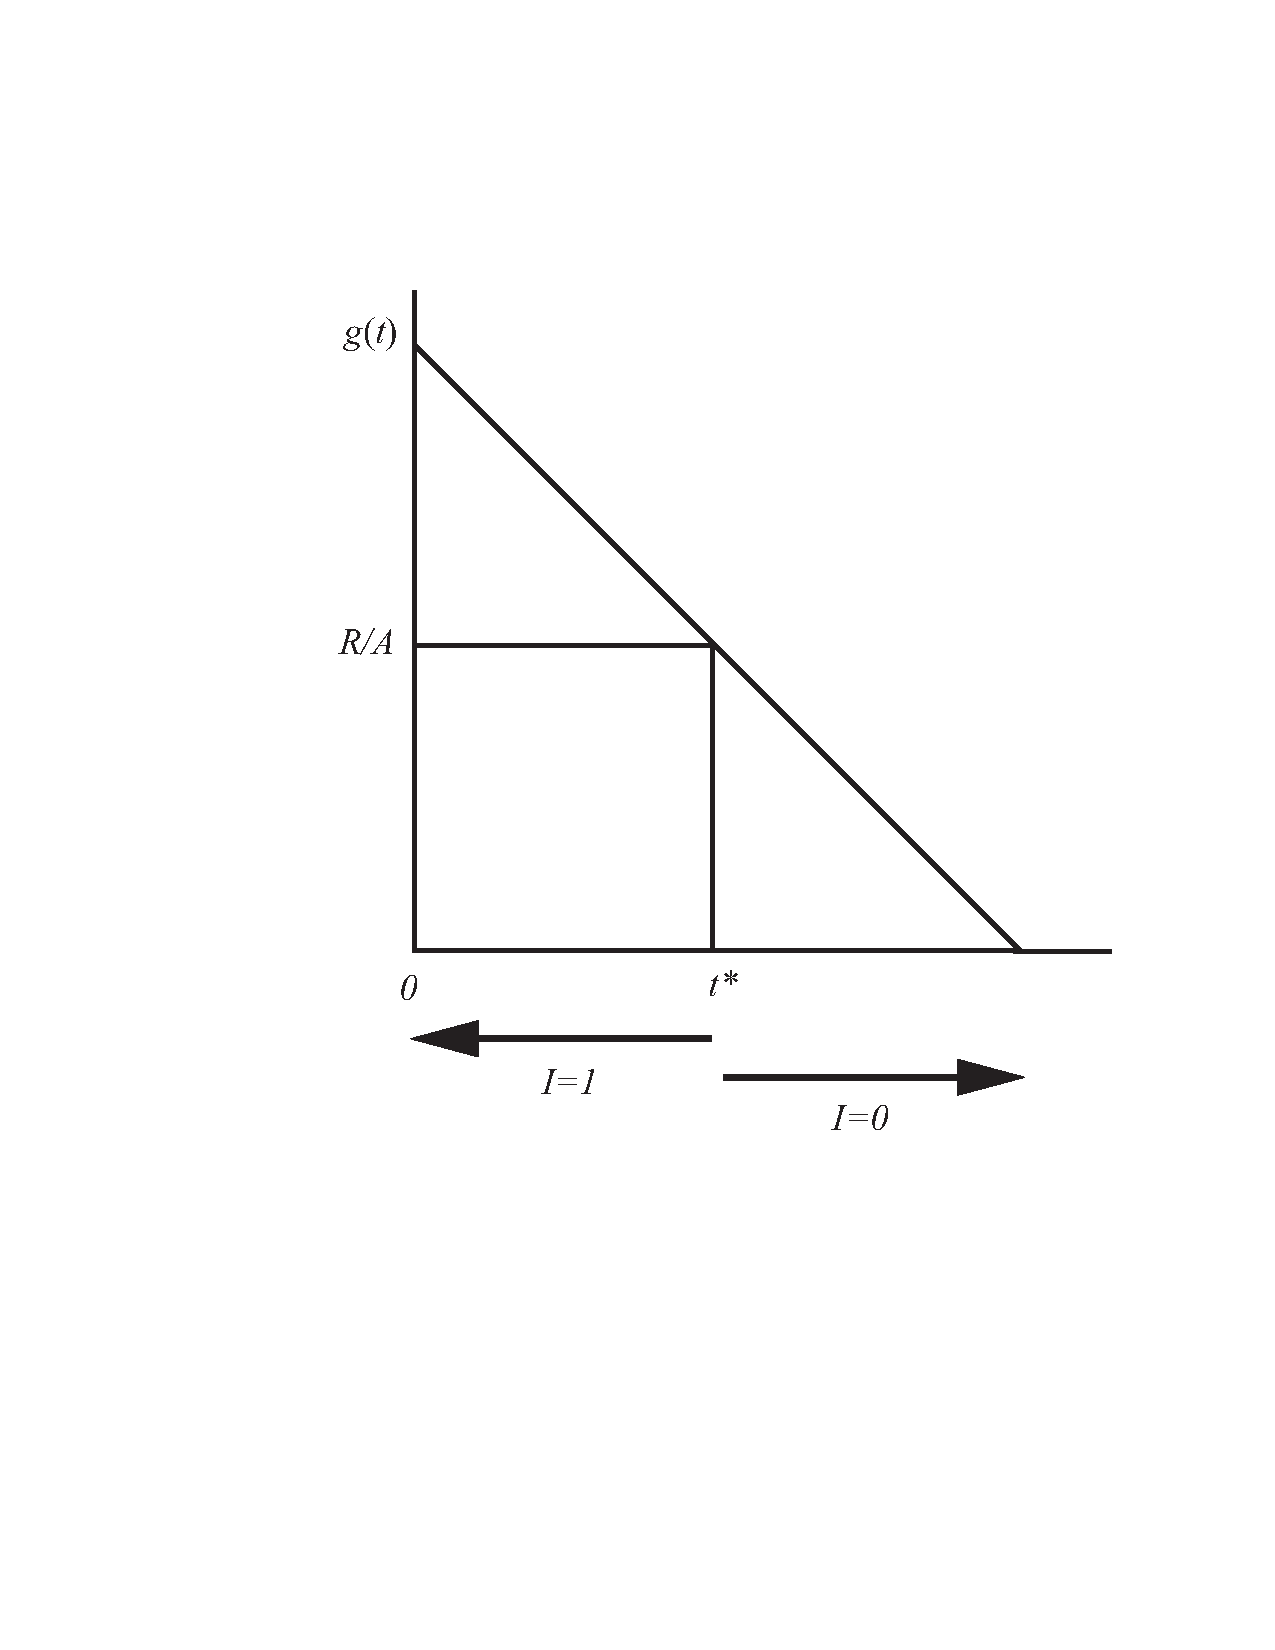
\includegraphics[width=3.2in]{include/fig-shesh-rule.pdf}
\end{center}
\end{frame}


%%%%%%%%%%%%%%%%%%%%%%%%%%%%%%%%%%%%%%%%%%%%%%%%%%%%%%%%%%%%%%%%%%%%%%%%%%%%%%%
\begin{frame}
\begin{itemize}[<+->]
\item At switching age $t^{*}$,
\begin{gather*}
\frac RA=\frac{1}{\sigma +r}\left(1-e^{(\sigma +r)(t^{*}-T)}\right) \\
\\
t^{*}=T+\frac{1}{\sigma +r}-\dfrac 1A
\end{gather*}
$t^{*}$ is schooling.
\bigskip

\item $T\uparrow \Rightarrow t^{*} \uparrow $

\item $\sigma ,r\uparrow \Rightarrow t^{*} \downarrow $

\item $A\uparrow \Rightarrow t^{*} \uparrow $

\item Initial endowments don't affect schooling.
\end{itemize}
\end{frame}


%%%%%%%%%%%%%%%%%%%%%%%%%%%%%%%%%%%%%%%%%%%%%%%%%%%%%%%%%%%%%%%%%%%%%%%%%%%%%%%
\begin{frame}
\begin{itemize}[<+->]
\item For $t\in [0,t^{*}]$,
\begin{align*}
\frac{\dot{H}}H=& (A-\sigma )t+\varphi, \qquad H(0)=H_0 \\[2mm]
H(t)=& e^{(A-\sigma )t}H(0).
\end{align*}

\item Human capital at schooling age $t^{*}$ is
\begin{equation*}
H(t^{*})=H(0)e^{(A-\sigma )}\left(T+\frac{1}{\sigma
+r}-\frac{1}{A}\right).
\end{equation*}

\item Coefficient on schooling: Mincer's ``$r$'' is $(A - \sigma)$
\begin{equation*}
\begin{array}{rcl@{\hspace{0in}}cl}
Y(t^{*}) &=& RH(0)H(t^{*}) & & \\[2mm]
\ln Y(t^{*}) &=& \ln RH(0)+(A-\sigma ) & t^{*} & \\
& & & \uparrow & \\
& & & \multicolumn{2}{l}{\text{years of school}}
\end{array}
\end{equation*}
\end{itemize}
\end{frame}


%%%%%%%%%%%%%%%%%%%%%%%%%%%%%%%%%%%%%%%%%%%%%%%%%%%%%%%%%%%%%%%%%%%%%%%%%%%%%%%
\section{Interior Sheshinski Specification}
%%%%%%%%%%%%%%%%%%%%%%%%%%%%%%%%%%%%%%%%%%%%%%%%%%%%%%%%%%%%%%%%%%%%%%%%%%%%%%%
\begin{frame}
\begin{center}
\textbf{\insertsection}
\end{center}
\begin{itemize}[<+->]
\item Now consider $0<\alpha <1$:
\begin{gather*}
\dot{H}=AI^\alpha H-\sigma H \\[2mm]
g(t)=\mu e^{rt} \\[2mm]
\mathcal{H}=e^{-rt}R(1-I)H+\mu (AI^\alpha H-\sigma H)
\end{gather*}

\item Therefore, if $g(t)\geq \dfrac{R}{A}$, person invests, full time $I =
    1$.
\item We get Sheshinski-like policy:
\begin{equation*}
\dot{g}=(\sigma +r-A)g
\end{equation*}

\item Need $(\sigma +r-A)<0$ to satisfy optimality of investment
    ($g(T)=0$).
\end{itemize}
\end{frame}


%%%%%%%%%%%%%%%%%%%%%%%%%%%%%%%%%%%%%%%%%%%%%%%%%%%%%%%%%%%%%%%%%%%%%%%%%%%%%%%
\section[Interior]{Interior Solution Case}
%%%%%%%%%%%%%%%%%%%%%%%%%%%%%%%%%%%%%%%%%%%%%%%%%%%%%%%%%%%%%%%%%%%%%%%%%%%%%%%
\begin{frame}
\begin{center}
\textbf{\insertsection}
\end{center}
\begin{itemize}[<+->]
\item We have
\begin{gather*}
RH=\alpha g(t)AI^{\alpha -1}H \\[2mm]
\dot{g}=-R(1-I)-gAI^{\alpha} +(\sigma +r)g
\end{gather*}

\item Now
\begin{equation*}
g(t)=\int_t^Te^{-(\sigma +r)(t-\tau
)}[(R)\underset{\begin{array}{c}\text{\small cash}\\
\text{\small
flow}\end{array}}{\underbrace{(1-I)}}+\underset{\begin{array}{c}\text{\small
future}\\ \text{\small
productivity}\end{array}}{\underbrace{gAI^{\alpha}}}\hspace{-.2in}]\,d\tau
\end{equation*}
\end{itemize}
\end{frame}


%%%%%%%%%%%%%%%%%%%%%%%%%%%%%%%%%%%%%%%%%%%%%%%%%%%%%%%%%%%%%%%%%%%%%%%%%%%%%%%
\begin{frame}
\begin{itemize}[<+->]
\item $I$ is obtained from the first order condition:
\begin{equation*}
I = \left[ \frac R{\alpha g(t)A}\right] ^{\frac 1{\alpha -1}} =
\left[ \frac{\alpha g(t)A}R\right] ^{\frac 1{1-\alpha }}
\end{equation*}
\begin{eqnarray*}
\dot{g} &=& -R\left( 1-\left( \frac{\alpha A}R\right) ^{\frac
1{1-\alpha }}g(t)^{\frac 1{1-\alpha }}\right) \\
&&-gA\left( \frac{\alpha A}R\right) ^{\frac \alpha {1-\alpha
}}g^{\frac \alpha {1-\alpha }}+(\sigma +r)g \\
\\
&=& -R+(g)^{\frac 1{1-\alpha }}\varphi +(\sigma +r)g
\end{eqnarray*}
\end{itemize}
\end{frame}


%%%%%%%%%%%%%%%%%%%%%%%%%%%%%%%%%%%%%%%%%%%%%%%%%%%%%%%%%%%%%%%%%%%%%%%%%%%%%%%
\begin{frame}
\begin{equation*}
\dot{g} = -R+(g)^{\frac 1{1-\alpha }}\varphi +(\sigma +r)g,
\end{equation*}
where
\begin{eqnarray*}
\varphi &=& R\left( \frac{\alpha A}R\right) ^{\frac 1{1-\alpha
}}-A\left( \frac{\alpha A}R\right) ^{\frac \alpha {1-\alpha }} \\
&=& (A)^{\frac 1{1-\alpha }}\left( \frac {\alpha}{R}\right) ^{\frac
\alpha {1-\alpha }}(\alpha -1)<0.
\end{eqnarray*}
When $\sigma +r=0$, $\dot{g}<0$ for sure.
\end{frame}


%%%%%%%%%%%%%%%%%%%%%%%%%%%%%%%%%%%%%%%%%%%%%%%%%%%%%%%%%%%%%%%%%%%%%%%%%%%%%%%
\begin{frame}
\begin{itemize}[<+->]
\item Note: Solution does not depend on initial conditions.

\item Case $\alpha =\frac{1}{2}$ produces Riccati equation:
\begin{equation*}
\dot{g}=-R+g^2\varphi +(\sigma +r)g
\end{equation*}

\item Solution: Let
\begin{gather*}
g^2\varphi +(\sigma +r)g-R=0 \\
(g-r_{+})(g-r_{-})=0
\end{gather*}

\item $r_{+}$ and $r_{-}$ are roots of equation (may be complex). Then, we
    can easily solve.
\end{itemize}
\end{frame}


%%%%%%%%%%%%%%%%%%%%%%%%%%%%%%%%%%%%%%%%%%%%%%%%%%%%%%%%%%%%%%%%%%%%%%%%%%%%%%%
\begin{frame}

\small

\begin{itemize}[<+->]
\item Suppose $r_{+}\neq r_{-}$ (distinct roots)
\begin{equation*}
\frac{g(t)-r_{+}}{g(t)-r_{-}}=c\ e^{\varphi (r_{+}-r_{-})t}
\end{equation*}

\item Transversality $\Rightarrow g(T) = 0 $. Therefore,
\begin{gather*}
\frac{r_{+}}{r_{-}}=ce^{\varphi (r_{+}-r_{-})T} \\
c=\left( \frac{r_{+}}{r_{-}}\right) e^{-\varphi (r_{+}-r_{-})T}
\end{gather*}

\item For $r_{+}=r_{-}=r_{0} \neq 0$ because $(\sigma +r)>0$, $R>0$;
\begin{gather*}
g(t)-r_0=\frac{1}{c-\varphi t} \\
g(t)=r_0 + \frac{1}{c-\varphi t} \\
g(T)=0 \Rightarrow c=\varphi T - y\frac{1}{r_0}
\end{gather*}
\end{itemize}

\end{frame}


%%%%%%%%%%%%%%%%%%%%%%%%%%%%%%%%%%%%%%%%%%%%%%%%%%%%%%%%%%%%%%%%%%%%%%%%%%%%%%%
\begin{frame}
\begin{itemize}[<+->]
\item Complex case is of economic interest.
\begin{equation*}
r_{\pm }=\frac{-(\sigma +r) \pm \sqrt{(\sigma +r)^{2}+4\varphi
R}}{2\varphi }
\end{equation*}
for $\alpha =\frac{1}{2}$, $\varphi =-(A)^2R^{-1}\frac{1}{4}$.

\item Therefore:
\begin{gather*}
(\sigma +r)^{2}-\frac{4R}4(A^{2})R^{-1} \\
(\sigma +r)^2-A^{2}, \text{ but } <0 \text{ from transversality}
\end{gather*}
\begin{eqnarray*}
r_{\pm } &=&\frac{-(\sigma +r)\pm \sqrt{(\sigma +r)^2-A^2}}{-\frac
12A^2R^{-1}} \\
&& \\
&=&\frac{+2R(\sigma +r)}{A^2}\mp \frac{2R\sqrt{(\sigma
+r)^2-A^2}}{A^2}.
\end{eqnarray*}
\end{itemize}
\end{frame}


%%%%%%%%%%%%%%%%%%%%%%%%%%%%%%%%%%%%%%%%%%%%%%%%%%%%%%%%%%%%%%%%%%%%%%%%%%%%%%%
\begin{frame}
\begin{itemize}[<+->]
\item
Now solution is very simple.\\[5mm]
\begin{gather*}
(g(t)-r_{+})=\left( \frac{r_{+}}{r_{-}}\right) e^{\varphi
(r_{+}-r_{-})(t-T)}(g(t)-r_{-}) \\
\\
g(t)\left[ 1-\frac{r_{+}}{r_{-}}e^{\varphi (r_{+}-r_{-})(t-T)}\right]
=r_{+}(1-e^{\varphi (r_{+}-r_{-})(t-T)}) \\
\\
g(t)=r_{+}\frac{1-e^{\varphi
(r_{+}-r_{-})(t-T)}}{1-\frac{r_{+}}{r_{-}}e^{\varphi (r_{+}-r_{-})(t-T)}}.
\end{gather*}
\end{itemize}
\end{frame}


%%%%%%%%%%%%%%%%%%%%%%%%%%%%%%%%%%%%%%%%%%%%%%%%%%%%%%%%%%%%%%%%%%%%%%%%%%%%%%%
\begin{frame}
\begin{itemize}[<+->]
\item Now,
\begin{equation*}
r_{+}=a+bi, \qquad r_{+}-r_{-}=(2bi), \qquad r_{-} = a - bi
\end{equation*}

\item Set $\theta =\varphi (2b)(t-T)$ (in radians)
\begin{eqnarray*}
g(t) &=&r_{+}\frac{(1-e^{i\theta })}{1-\frac{r_{+}}{r_{-}}e^{i\theta }} \\
&=&(r_{+}r_{-})\frac{(1-e^{i\theta })}{(r_{-}-r_{+}e^{i\theta })}
\end{eqnarray*}

\item $r_{+}r_{-}=a^2+b^2$. Now multiply by $e^{-i\theta /2}$,
\begin{equation*}
g(t)=(r_{+}r_{-})\frac{(e^{-i\theta /2}-e^{i\theta
/2})}{(r_{-}e^{-i\theta /2}-r_{+}e^{i\theta /2})}
\end{equation*}
\end{itemize}
\end{frame}


%%%%%%%%%%%%%%%%%%%%%%%%%%%%%%%%%%%%%%%%%%%%%%%%%%%%%%%%%%%%%%%%%%%%%%%%%%%%%%%
\begin{frame}
Using $\cos (-x)=\cos x\quad \sin (-x)=-\sin x$,
\begin{eqnarray*}
e^{ix}&=&\cos x+i\sin x \\
g(t)&=&(r_{+}r_{-})\left[ \frac{\cos (\theta /2)-i\sin \theta /2-\cos (\theta
/2)-i\sin \theta /2}{-2ai\sin \theta /2-2b_i\cos \theta /2}\right] \\
&=&(r_{+}r_{-})\left[ \frac{\sin \theta /2}{a\sin \theta /2+b\cos
\theta /2}\right] \\
&=&\left( \frac{r_{+}r_{-}}a\right) \left[ \frac 1{1+\dfrac ba\cot
\theta /2}\right]
\end{eqnarray*}
Therefore,
\begin{equation*}
g(t) =\frac{(a^2+b^2)}a\left[ \frac 1{1+\dfrac ba\cot \varphi
b(t-T)}\right]
\end{equation*}
\end{frame}


%%%%%%%%%%%%%%%%%%%%%%%%%%%%%%%%%%%%%%%%%%%%%%%%%%%%%%%%%%%%%%%%%%%%%%%%%%%%%%%
\begin{frame}
\begin{gather*}
a=\frac{2(\sigma+r)R}{A^2} \qquad \quad
b=\frac{2R}{A^2}(A^2-(\sigma+r)^2)^{1/2}\\
\varphi b =-\frac 12(A^2-(\sigma ^2+r^2))^{1/2} \\
\\
\frac ba =\frac{2R(A^2-(\sigma ^2+r^2))^{1/2}/A^2}{2\dfrac{(\sigma +r)R}{A^2}}
=\dfrac{[A^2-(\sigma ^2+r^2)]^{1/2}}{\sigma +r}
\end{gather*}

When $\sigma +r=0$,
\begin{equation*}
r_{\pm } =\pm \frac{\sqrt{4\varphi R}}{2\varphi }=\pm \sqrt{\frac{R}{\varphi}}
=\pm \sqrt{\frac{4R}{-A^2R^{-1}}} =\left( \frac{2R}A\right) i
\end{equation*}

\begin{equation*}
\varphi b =\left[ -(A)^2\dfrac{R^{-1}}4\right] \left[ \dfrac{2R}{A^2} A\right]
=-\dfrac A2
\end{equation*}
\end{frame}


%%%%%%%%%%%%%%%%%%%%%%%%%%%%%%%%%%%%%%%%%%%%%%%%%%%%%%%%%%%%%%%%%%%%%%%%%%%%%%%
\begin{frame}
\begin{eqnarray*}
g(t) &=&\left( \dfrac{4R^2}{A^2}\right) \frac{\tan
}{\dfrac{2R}{A^2}A}(\theta /2) \\
&=&\left( \dfrac{2R}A\right) \tan \left[ \frac \theta 2\right] \\
&=&\left( \dfrac{2R}A\right)\tan \left( -\frac A2(t-T)\right) \\
&=&\left( \frac{2R}A\right) \tan \left( \frac A2(T-t)\right)
\end{eqnarray*}

\begin{itemize}[<+->]
\item From definition of $\theta$, we obtain
\begin{equation*}
g(t)=\left(\frac{2R}{A}\right)\tan \left( \frac{A}{2}(T-t)\right)
\end{equation*}
\end{itemize}
\end{frame}


%%%%%%%%%%%%%%%%%%%%%%%%%%%%%%%%%%%%%%%%%%%%%%%%%%%%%%%%%%%%%%%%%%%%%%%%%%%%%%%
\section{Modified Sheshinski Specification}
%%%%%%%%%%%%%%%%%%%%%%%%%%%%%%%%%%%%%%%%%%%%%%%%%%%%%%%%%%%%%%%%%%%%%%%%%%%%%%%
\begin{frame}
\begin{center}
\textbf{\insertsection\ (More Interesting)}
\end{center}
\begin{gather*}
\dot{H}=AI-\sigma \\
\\
\mathcal{H}=e^{-rt}R(1-I)H+\mu (t)(AI-\sigma H)
\end{gather*}

\begin{itemize}[<+->]
\item $I=1$ if $\mu A \geq e^{-rt}R$
\item $I=0$ otherwise
\end{itemize}
\end{frame}


%%%%%%%%%%%%%%%%%%%%%%%%%%%%%%%%%%%%%%%%%%%%%%%%%%%%%%%%%%%%%%%%%%%%%%%%%%%%%%%
\begin{frame}
\begin{gather*}
g(t)=\mu (t)e^{rt} \\
\dot{g}=-R(1-I)+g(\sigma +r) \\
g(t)=R\int_t^T e^{+(\sigma +r)(t-\tau )}(1-I)\,d\tau \\
g\geq \frac{R}{A}H,\qquad I=1
\end{gather*}
\begin{itemize}[<+->]
\item When $I=1$, $\dot{g}=g(\sigma +r)>0$ and g$\uparrow $
\item Intuition: as $t\uparrow $ agent is getting nearer the payoff period.
\item While the agent invests he/she gets no return.
\end{itemize}
\end{frame}


%%%%%%%%%%%%%%%%%%%%%%%%%%%%%%%%%%%%%%%%%%%%%%%%%%%%%%%%%%%%%%%%%%%%%%%%%%%%%%%
\begin{frame}
\begin{itemize}[<+->]
\item First take case when $\sigma =0$
  \begin{equation*}
    \dot{g}= -R(1-I)+rg
  \end{equation*}

\item For $t=0$, if $g(t)\geq \frac{R}{A}H(t)$; $I=1$; $\dot{H}=A$,
  \begin{equation*}
    H(t)=At+H(0)
  \end{equation*}
\item Let $\hat{t}$ be the age of the first interior solution.
\item At $\hat{t}$, $g(\hat{t})=\frac{R}{A}H(\hat{t})$,
  \begin{equation*}
    g(0)e^{r\hat{t}}=\frac{R}{A}[A\hat{t}+H(0)]
  \end{equation*}
\end{itemize}
\end{frame}


%%%%%%%%%%%%%%%%%%%%%%%%%%%%%%%%%%%%%%%%%%%%%%%%%%%%%%%%%%%%%%%%%%%%%%%%%%%%%%%
\begin{frame}
\begin{itemize}[<+->]
\item Observe that
  \begin{equation*}
  g(t) \leq R\int_t^T e^{+(\sigma +r)(t-\tau )}\,d\tau
  \end{equation*}
  (i.e.\ set $I(\tau) = 0$).

\item Therefore, $g(t) \leq \frac{R}{\sigma +r}\left(1- e^{+(\sigma
    +r)(t-\tau )} \right) \leq \frac{R}{\sigma + r}$

\item Therefore, $\dot{g} < 0$ (after the period of investment)

\item Thus at most one period of specialization and it comes at the
    beginning of life if at all. Will not arise if $g(0) < \frac{R}{A}$,
    i.e.\ $A < r$ precludes this (return by investment $<$ return by saving
    in lending market.
\item This is a model of schooling.
\end{itemize}
\end{frame}


%%%%%%%%%%%%%%%%%%%%%%%%%%%%%%%%%%%%%%%%%%%%%%%%%%%%%%%%%%%%%%%%%%%%%%%%%%%%%%%
\begin{frame}
\begin{itemize}[<+->]
\item Therefore, $t^{*}$ is solution from
  \begin{eqnarray*}
    \frac{R}{r}\left(1- e^{r(t^{*}-T)}\right) &=& \frac{R}{A}(At^{*}+H_{0}) \\
    \\
    \left(1- e^{r(t^{*}-T)}\right) &=& \frac{r}{A}(At^{*}+H_{0})
  \end{eqnarray*}

\item The higher $H_{0}$, the lower $t^{*}$.
\item Need $r<A$ for feasibility.

\item Human capital stock at end of school:
  \begin{gather*}
    H = At^{*}+H_{0} \\
    Y(t^{*}) = R(At^{*}+H_{0})
  \end{gather*}
\end{itemize}
\end{frame}


%%%%%%%%%%%%%%%%%%%%%%%%%%%%%%%%%%%%%%%%%%%%%%%%%%%%%%%%%%%%%%%%%%%%%%%%%%%%%%%
\begin{frame}
\begin{itemize}[<+->]
\item Take case where $\sigma > 0$. Now, by the previous logic, $g \leq
    \frac{R}{\sigma + r}$.
\item Therefore, $\dot{g} < 0$.

\item Now investment pattern \emph{may} be more complex.

\item Suppose $g(0) \geq \frac{R}{A}H(0)$. Then $I(0) = 1$.
  \begin{gather*}
    \frac{\dot{g}}{g} = (\sigma + r) \\
    \dot{H} = A - \sigma H
  \end{gather*}
  \begin{eqnarray*}
    H(t) &=& A \int_{0}^{t} e^{-\sigma (t - \tau)}\,d\tau + H(0)e^{-\sigma t} \\
     &=& \frac{A}{\sigma} (1 - e^{-\sigma t}) + H(0)e^{-\sigma t} \\
     &=& \frac{A}{\sigma} + \left[H(0) - \frac{A}{\sigma} \right] e^{-\sigma t}
  \end{eqnarray*}
\end{itemize}
\end{frame}


%%%%%%%%%%%%%%%%%%%%%%%%%%%%%%%%%%%%%%%%%%%%%%%%%%%%%%%%%%%%%%%%%%%%%%%%%%%%%%%
\begin{frame}
\begin{itemize}[<+->]
\item
  \begin{eqnarray*}
    g(0) e^{(\sigma + r)\hat{t}} &=& \frac{R}{A} \left( \frac{A}{\sigma}(1- e^{-\sigma \hat{t}}) + H(0)e^{-\sigma \hat{t}} \right) \\
     &=& R \left(\frac{H(0)}{A} - \frac{1}{\sigma} \right)e^{-\sigma \hat{t}} + \frac{R}{\sigma}
  \end{eqnarray*}

\item To ensure $\dot{H} > 0$ at $t=0$, need $A - \sigma H(0) >0
    \Rightarrow A > \sigma H(0) \Rightarrow \frac{1}{\sigma} >
    \frac{H(0)}{A}$.
\end{itemize}
\end{frame}


%%%%%%%%%%%%%%%%%%%%%%%%%%%%%%%%%%%%%%%%%%%%%%%%%%%%%%%%%%%%%%%%%%%%%%%%%%%%%%
\begin{frame}
\frametitle{For intersection to occur, we have:}
\begin{center}
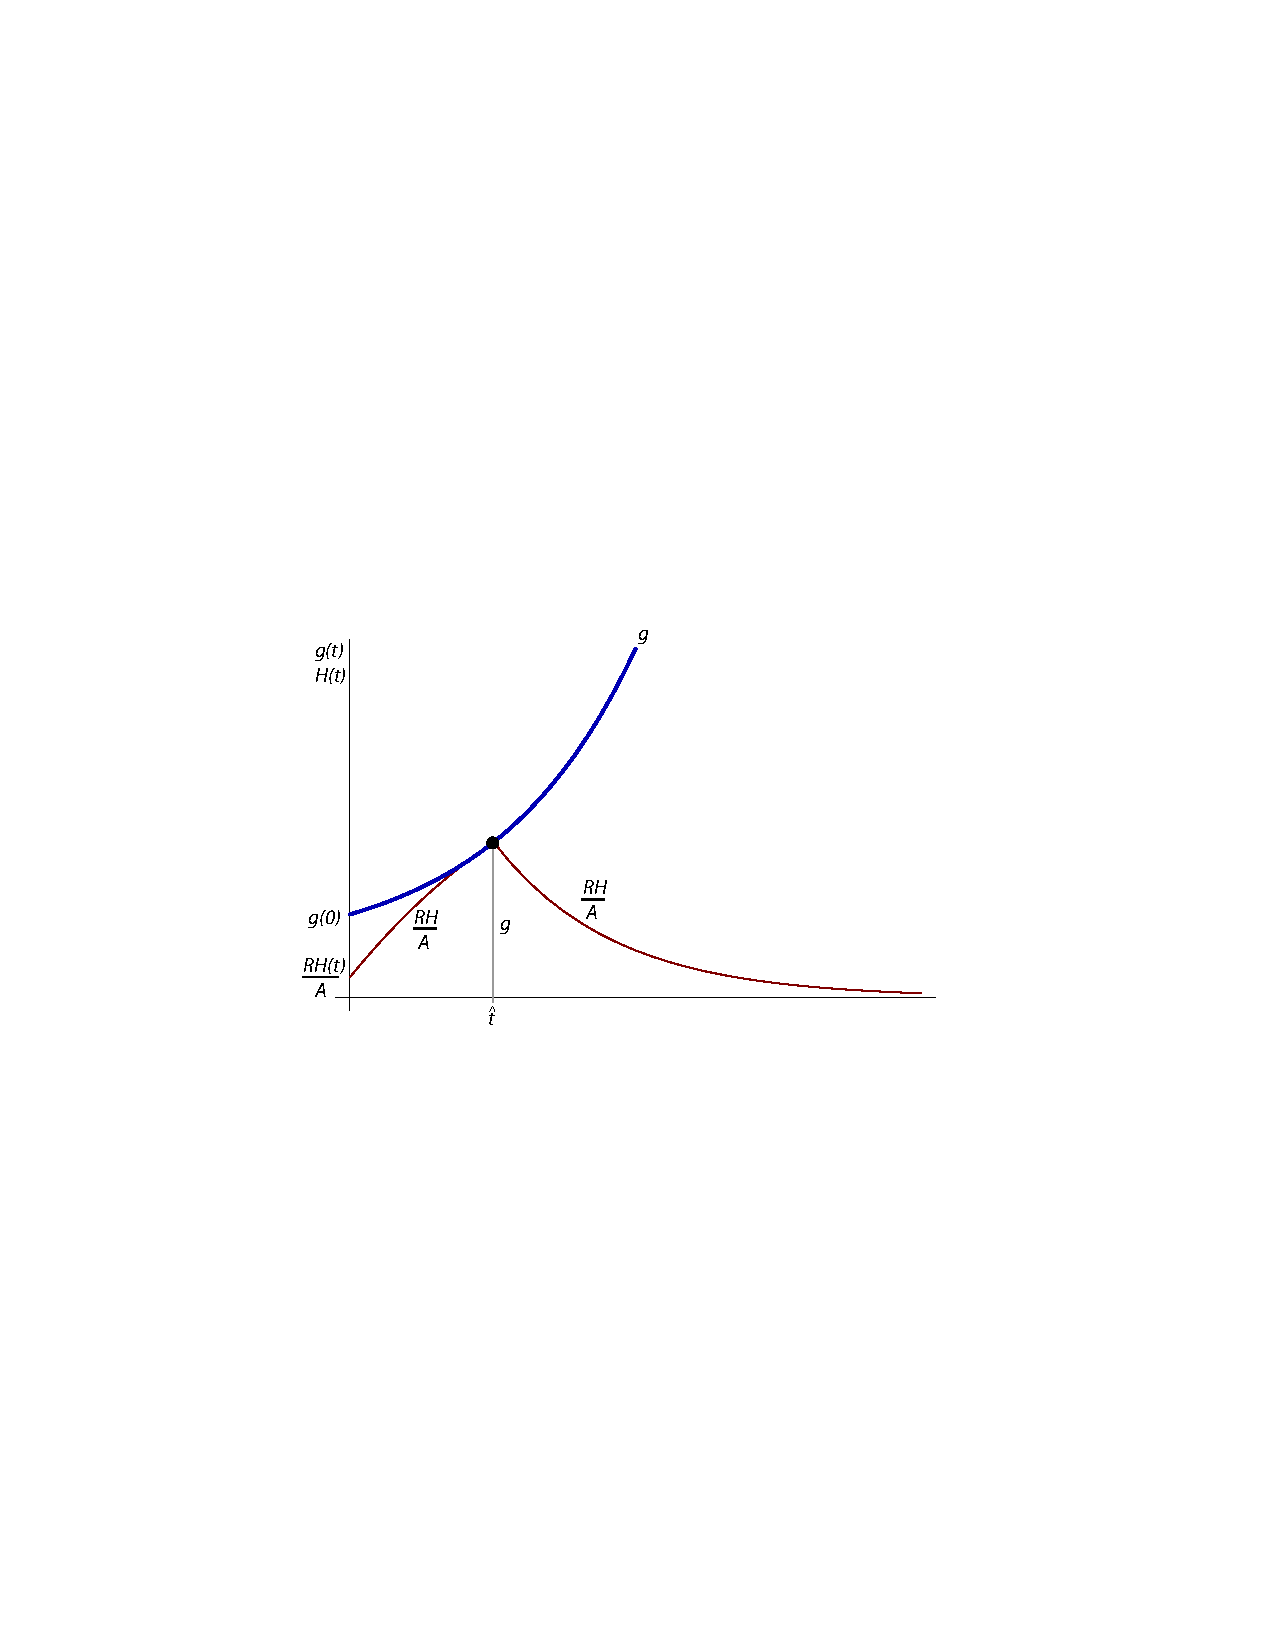
\includegraphics[width=4in]{include/fig-shesh-for-intersection}
\end{center}
\end{frame}


%%%%%%%%%%%%%%%%%%%%%%%%%%%%%%%%%%%%%%%%%%%%%%%%%%%%%%%%%%%%%%%%%%%%%%%%%%%%%%%
\begin{frame}
\begin{itemize}[<+->]
\item
  \begin{gather*}
    g(0) \geq \frac{R}{A} H(0) \\
    H(t) = \frac{A}{\sigma} + \left[ H(0) - \frac{A}{\sigma} \right]
    e^{-\sigma t}
  \end{gather*}

\item $t_{1}$ is the first point where $g(t_{1}) = \frac{R}{A} H(t_{1})$

\item $\dot{g}(t) = (\sigma + r)g$ so $g(t_{1}) = e^{(\sigma +
    r)t_{1}}g(0)$.

\item Then,
  \begin{equation*}
    \frac{R}{\sigma} + \frac{R}{A} \left[ H(0) - \frac{A}{\sigma}
    \right] e^{-\sigma t_{1}} = g(0)e^{(\sigma + r)t_{1}}.
  \end{equation*}
\end{itemize}
\end{frame}


%%%%%%%%%%%%%%%%%%%%%%%%%%%%%%%%%%%%%%%%%%%%%%%%%%%%%%%%%%%%%%%%%%%%%%%%%%%%%%%
\begin{frame}
\begin{itemize}[<+->]
\item Then at $t_{1}$, $I=0$,
  \begin{eqnarray*}
    \dot{g} &=& -R +(\sigma +r)g \\
    H(t) &=& H(t_{1}) e^{-\sigma (t -t_{1})} \qquad t_{1} < t < t_{2} \\
    g(t) &=& \frac{R}{\sigma +r} \left( 1 -e^{+(\sigma +r)(t -t_{2})} \right)+g(t_{2})e^{(\sigma +r)(t -t_{2})}
  \end{eqnarray*}

\item At $t_{2}$, we have that
  \begin{eqnarray*}
    \frac{R H(t_{2})}{A} &=& RH(t_{1})e^{-\sigma (t_{2}-t_{1})} \\
     &=& g(t_{2}) = \int_{t_{2}}^{T} e^{-(\sigma +r)(t_{2}-\tau)} (1 -I(\tau))\,d\tau
  \end{eqnarray*}

\item Then person bangs in at $I=1$ and, possibly a sequence of intervals
    of specialization.

\item $t_{2} < t < t_{3}$; etc.
\end{itemize}
\end{frame}


%%%%%%%%%%%%%%%%%%%%%%%%%%%%%%%%%%%%%%%%%%%%%%%%%%%%%%%%%%%%%%%%%%%%%%%%%%%%%%
\begin{frame}
\frametitle{One possible trajectory}

\begin{center}
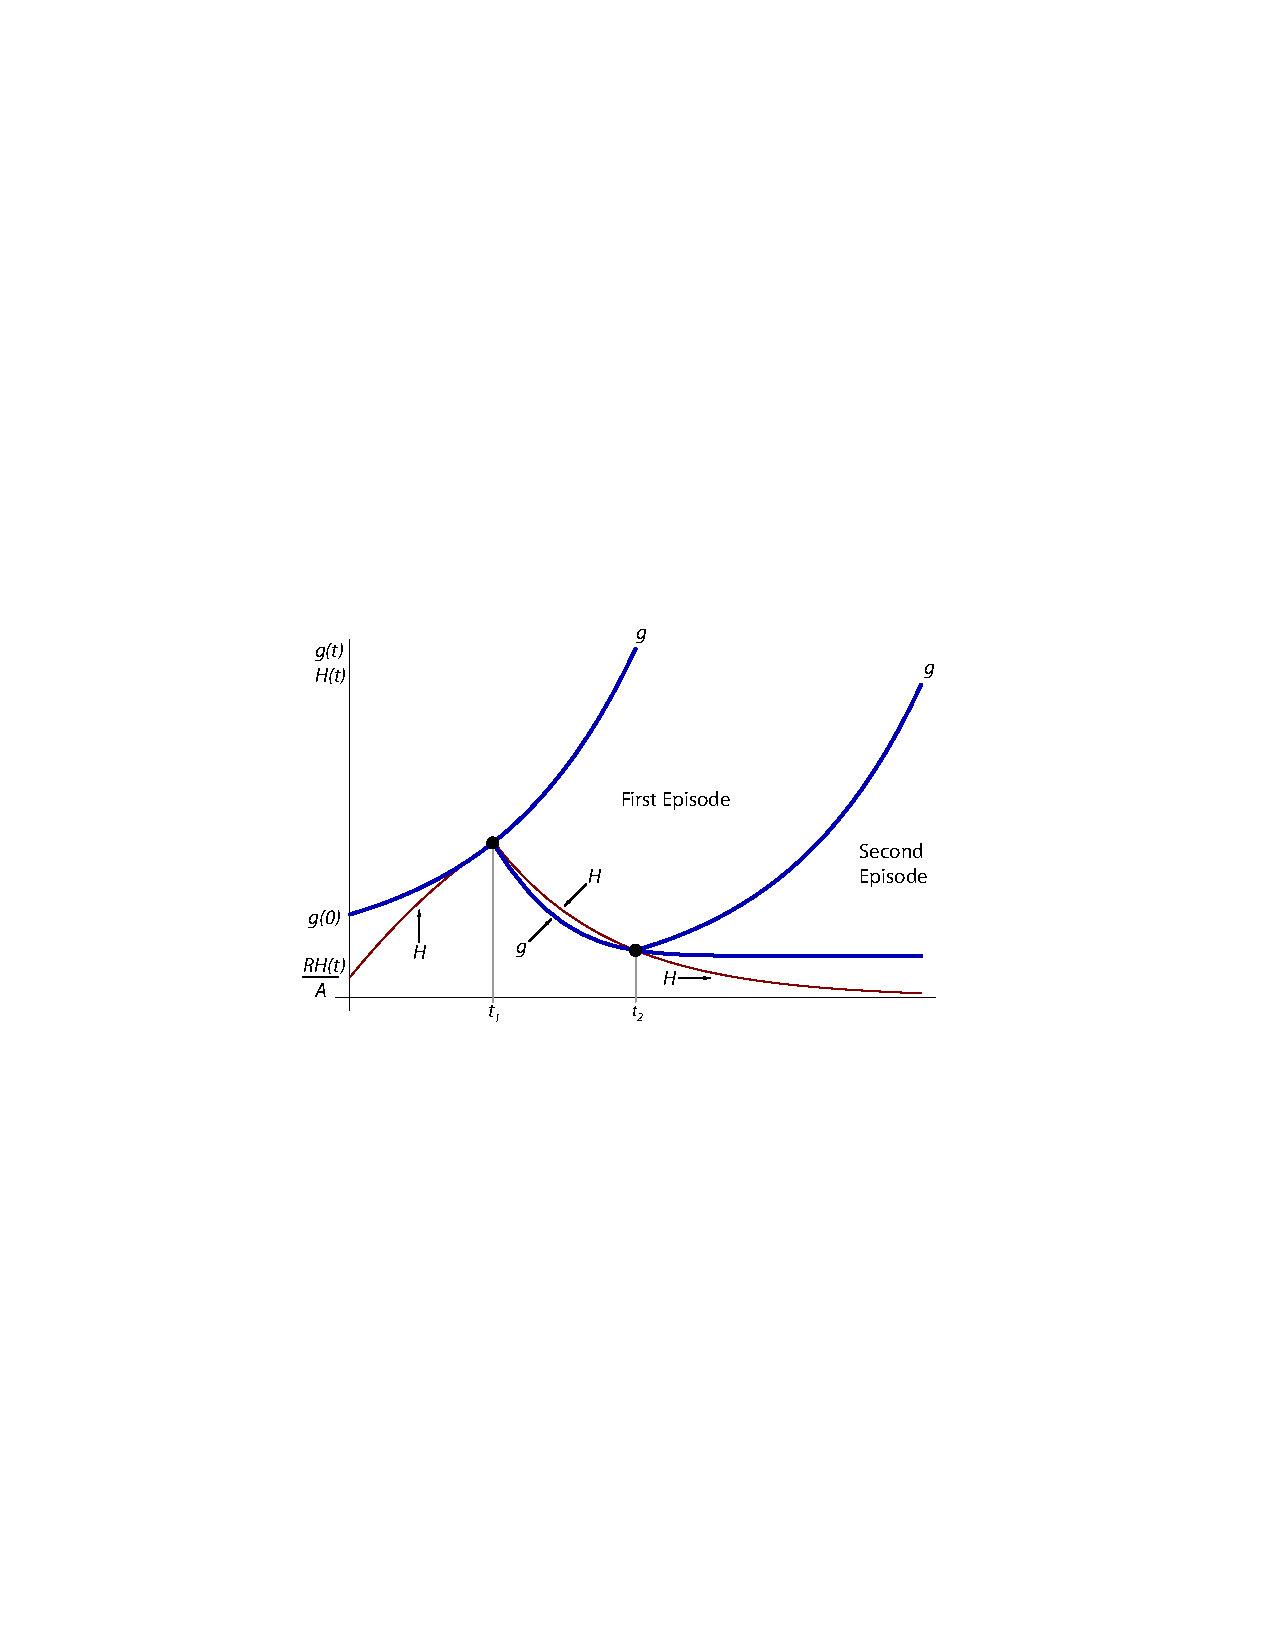
\includegraphics[width=4in]{include/fig-shesh-one-traj}
\end{center}

\end{frame}


%%%%%%%%%%%%%%%%%%%%%%%%%%%%%%%%%%%%%%%%%%%%%%%%%%%%%%%%%%%%%%%%%%%%%%%%%%%%%%%
\begin{frame}
\begin{itemize}[<+->]
\item We could also have one shot indefinitely (but last shots are
    ``short'').

\item Observe:
  \begin{equation*}
    g(t) = R \int_{t_{1}}^{t_{2}} e^{(\sigma +r)(t-\tau)}\,d\tau
    + \dots + \int_{t_{3}}^{t_{4}} e^{(\sigma +r)(t-\tau)}\,d\tau
    + \cdots
  \end{equation*}
\end{itemize}

\end{frame}


%%%%%%%%%%%%%%%%%%%%%%%%%%%%%%%%%%%%%%%%%%%%%%%%%%%%%%%%%%%%%%%%%%%%%%%%%%%%%%%
\begin{frame}
\begin{itemize}[<+->]
\item For $t<t_{1}$, $t\uparrow$, $g\uparrow$ can happen.

\item For this to occur:
  \begin{itemize}[<+->]
    \item In a neighborhood of $t_{1}$:
    \begin{equation*}
      \dot{g}(t_{1}) < \left. \frac{R\dot{H}(t)}{A} \right|_{t=t_{1}}
    \end{equation*}
    (demand price less than opportunity cost).

    \item The curves must cross. Otherwise, we get failure of
        transversality.
    \end{itemize}
\end{itemize}
\end{frame}


%%%%%%%%%%%%%%%%%%%%%%%%%%%%%%%%%%%%%%%%%%%%%%%%%%%%%%%%%%%%%%%%%%%%%%%%%%%%%%%
\begin{frame}
\begin{itemize}[<+->]
\item Whether or not such investment activity occurs depends on initial
    $H(0)$ and other parameters.

\item Thus, at time $t_{1}$, for this to arise, we need:
  \begin{equation*}
    \dot{g}\bigg|_{t=t_{1}} < \left. \frac{R\dot{H}(t)}{A}
    \right|_{t=t_{1}}.
  \end{equation*}

\item $g$ is continuous at $t_{1}$ (but not necessarily differentiable and,
    in our case, definitely not).
\end{itemize}
\end{frame}


%%%%%%%%%%%%%%%%%%%%%%%%%%%%%%%%%%%%%%%%%%%%%%%%%%%%%%%%%%%%%%%%%%%%%%%%%%%%%%%
\begin{frame}
\begin{itemize}[<+->]
\item At $t_{1}$, $g(t_{1})=\frac{R}{A}H(t_{1})$
  \begin{gather*}
    \dot{g} = -R + (\sigma +r)g \qquad \text{(from right)} \\
    \\
    \frac{R}{A}\dot{H}(t_{1}) = -\sigma\frac{R}{A}H(t_{1}) = -\sigma
    g(t_{1})
  \end{gather*}

\item Therefore, we need:
  \begin{equation*}
    -R + (\sigma +r)g(t_{1}) < -\sigma g(t_{1}) = \left. \frac{R\dot{H}(t)}{A}
    \right|_{t=t_{1}}
  \end{equation*}
\item However, this is not guaranteed by $\frac{R}{\sigma +r}>g$. We need a
    tighter bound.
\end{itemize}
\end{frame}


%%%%%%%%%%%%%%%%%%%%%%%%%%%%%%%%%%%%%%%%%%%%%%%%%%%%%%%%%%%%%%%%%%%%%%%%%%%%%%%
\begin{frame}
\begin{itemize}[<+->]
\item For specialization to occur at $0$, we need:
  \begin{equation*}
    g(0) \geq \frac{R}{A}H(0),
  \end{equation*}
  but we need the slope of $\left. \frac{RH(t)}{A} \right|_{t=0}$ to exceed
  $\dot{g}\bigg|_{t=0}$ (otherwise, $g$ curve and $\frac{R}{A}H(t)$ curves
  do not intersect).
\\[2mm]

\item For the required condition we need (using expression for $RH(t)$ in a
    neighborhood of $t=0$):
  \begin{equation*}
    R \left( 1 -\frac{\sigma H(0)}{A} \right) > g(0)(\sigma +r)
  \end{equation*}
\end{itemize}
\end{frame}


%%%%%%%%%%%%%%%%%%%%%%%%%%%%%%%%%%%%%%%%%%%%%%%%%%%%%%%%%%%%%%%%%%%%%%%%%%%%%%%
\begin{frame}
\begin{itemize}[<+->]
\item Sufficient condition:
  \begin{equation*}
    \left( 1 -\frac{\sigma H(0)}{A} \right) \geq 1 -e^{(\sigma +r)T}
  \end{equation*}
  (but this is way too strong)

  \medskip

\item Necessary condition:
  \begin{equation*}
    \frac{\sigma H(0)}{A} < 1
  \end{equation*}
  (otherwise, never pays to specialize)

  \medskip

\item Therefore, if $H(0)$ is too high, agent never specializes.

  \medskip

\item At $g(0)$, we must have:
  \begin{equation*}
    \frac{R}{\sigma +r} \left( 1 -\frac{\sigma H(0)}{A} \right) >
    g(0) > \frac{R H(0)}{A}.
  \end{equation*}
  If $H(0)$ big enough, cannot happen.
\end{itemize}
\end{frame}


%%%%%%%%%%%%%%%%%%%%%%%%%%%%%%%%%%%%%%%%%%%%%%%%%%%%%%%%%%%%%%%%%%%%%%%%%%%%%%%
\begin{frame}
Observe that:
\begin{equation*}
    g(t) = R\int_t^T e^{-(\sigma +r)(t-\tau )}(1-I(\tau))\,d\tau
\end{equation*}

Recall that $I$ switches between 0 and 1. Therefore:
\begin{itemize}[<+->]
\item For $0 < t < t_{1}$ (person invests),
  \begin{equation*}
    g(t) = {\textstyle \frac{R}{\sigma +r}} e^{(\sigma +r)t}
    \sum_{k \geq 1} (-1)^{k+1} e^{-(\sigma +r)t_{k}}
  \end{equation*}

\item For $t_{1} < t < t_{2}$ (person does not invest),
  \begin{equation*}
    g(t) = {\textstyle \frac{R}{\sigma +r}} \left[1 - e^{(\sigma +r)(t-t_{2})}\right]
    + {\textstyle \frac{R}{\sigma +r}} e^{(\sigma +r)t}
    \sum_{k \geq 3} (-1)^{k+1} e^{-(\sigma +r)t_{k}}
  \end{equation*}

\item For $t_{2} < t < t_{3}$ (etc.),
  \begin{equation*}
    g(t) = {\textstyle \frac{R}{\sigma +r}} e^{(\sigma +r)t}
    \sum_{k \geq 3} (-1)^{k+1} e^{-(\sigma +r)t_{k}}
  \end{equation*}
\end{itemize}
\end{frame}


%%%%%%%%%%%%%%%%%%%%%%%%%%%%%%%%%%%%%%%%%%%%%%%%%%%%%%%%%%%%%%%%%%%%%%%%%%%%%%%
\begin{frame}
\begin{itemize}[<+->]
\item Cannot prove that $g(t_{3}) < g(t_{1})$ for all policies.
\\[2mm]

\item Person may build up stock of human capital over the lifetime.
\end{itemize}
\end{frame}


\end{document}
